\documentclass{article}
\usepackage{spikey}
\usepackage{amsmath}
\usepackage{mathrsfs}
\usepackage{amssymb}
\usepackage{soul}
\usepackage{float}
\usepackage{graphicx}
\usepackage{hyperref}
\usepackage{fancyhdr}
\usepackage{xcolor}
\usepackage{chngcntr}
\usepackage{centernot}
\usepackage[shortlabels]{enumitem}
\usepackage[margin=1truein]{geometry}
\usepackage{tkz-graph}
\usepackage{dsfont}
\usepackage{caption}
\usepackage{subcaption}
\usepackage{booktabs}
\usepackage[yyyymmdd,hhmmss]{datetime}

\usepackage{tikz}
\usetikzlibrary{arrows}

\usepackage{setspace}
\linespread{1.15}
\usepackage[margin=1truein]{geometry}

\counterwithin{equation}{section}
\counterwithin{figure}{section}

\usepackage{listings}
 
\definecolor{codegreen}{rgb}{0,0.6,0}
\definecolor{codegray}{rgb}{0.5,0.5,0.5}
\definecolor{codeblue}{rgb}{0.3,0.5,0.8}
\definecolor{codepurple}{rgb}{0.58,0,0.82}
%\definecolor{backcolour}{rgb}{0.95,0.95,0.92}
\definecolor{backcolour}{rgb}{1,1,1}

\lstdefinestyle{mystyle}{
    backgroundcolor=\color{backcolour},   
    commentstyle=\color{codegreen},
    keywordstyle=\color{magenta},
    numberstyle=\tiny\color{codegray},
    stringstyle=\color{codepurple},
    basicstyle=\ttfamily\footnotesize,
    breakatwhitespace=false,         
    breaklines=true,                 
    captionpos=b,                    
    keepspaces=true,                 
    numbers=left,                    
    numbersep=5pt,                  
    showspaces=false,                
    showstringspaces=false,
    showtabs=false,                  
    tabsize=4
}

\lstset{style=mystyle}

\title{CSC413: Programming Assignment 3}
\date{\today\ at \currenttime}
\author{Tianyu Du (1003801647)}
\begin{document}
	\maketitle
	\section{Part 1: Gated Recurrent Units}
	\subsection{}
\begin{lstlisting}[language=python]
class MyGRUCell(nn.Module):
    def __init__(self, input_size, hidden_size):
        super(MyGRUCell, self).__init__()

        self.input_size = input_size
        self.hidden_size = hidden_size

        # ------------
        # FILL THIS IN
        # ------------
        ## Input linear layers
        self.Wiz = nn.Linear(input_size, hidden_size, bias=False)
        self.Wir = nn.Linear(input_size, hidden_size, bias=False)
        self.Win = nn.Linear(input_size, hidden_size, bias=False)

        ## Hidden linear layers
        self.Whz = nn.Linear(hidden_size, hidden_size, bias=True)
        self.Whr = nn.Linear(hidden_size, hidden_size, bias=True)
        self.Whn = nn.Linear(hidden_size, hidden_size, bias=True)
        

    def forward(self, x, h_prev):
        # ------------
        # FILL THIS IN
        # ------------
        r = torch.sigmoid(self.Wir(x) + self.Whr(h_prev))
        z = torch.sigmoid(self.Wiz(x) + self.Whz(h_prev))
        g = torch.tanh(self.Win(x) + r * self.Whn(h_prev))
        h_new = (1 - z) * g + z * h_prev
        return h_new
\end{lstlisting}
	\subsection{}
	\begin{figure}[H]
		\centering
		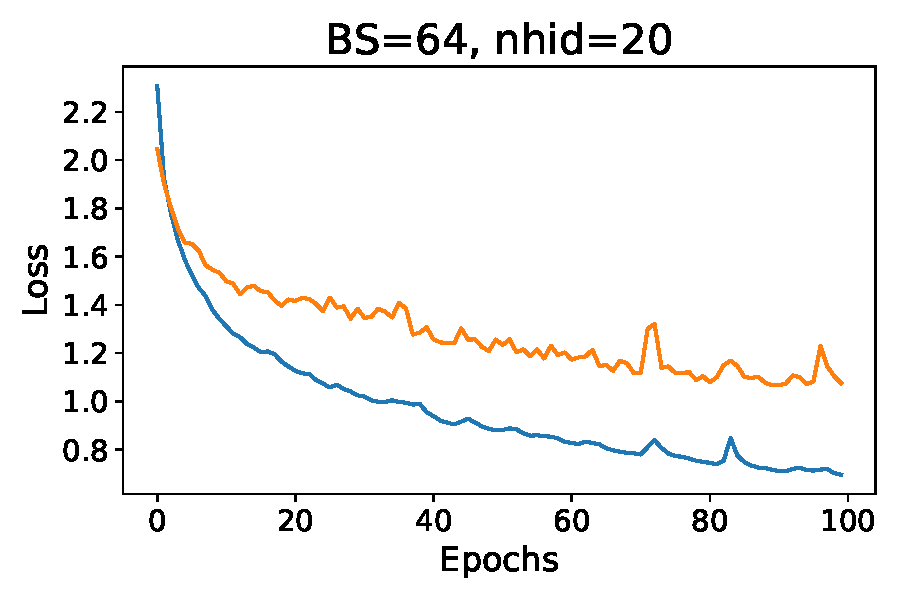
\includegraphics[width=0.7\linewidth]{GRU_loss_plot.pdf}
	\end{figure}
	\subsection{}
\paragraph{Failure Type 1} Long vocabularies. The model fails to translate long vocabularies, the middle part of vocabularies get messed up.
\begin{lstlisting}
source:		computer science 
translated:	opcorchyway ipenceway
\end{lstlisting}
\paragraph{Failure Type 2} Vocabularies containing dashes ("-"). The model fails to distinguish parts of word before and after the dash. Sometime, the dash is missing after translation.
\begin{lstlisting}
source:		electric-powered 
translated:	elcercorstentway
================================
source:		to-buy 
translated:	otay-othay
\end{lstlisting}
	
	\section{Additive Attention}
	\subsection{}
	\begin{align}
		\tilde{\alpha}_i^{(t)} &= f(Q_i, K_i) = W_2\ \tx{ReLU}(W_1 [Q_i, K_i] + b_1) + b_2\\
		\alpha_i^{(t)} &= \text{softmax}(\tilde{\alpha}^{(t)})_i = \frac{\exp(\tilde{\alpha}_i^{(t)})}{\sum_{t=1}^\texttt{seq\_len} \exp(\tilde{\alpha}_i^{(t)})} \\
		c_t &= \sum_{i	=1}^\texttt{seq\_len} \alpha_i^{(t)} K_i
	\end{align}
	\subsection{}
\begin{lstlisting}[language=python]
class RNNAttentionDecoder(nn.Module):
    def __init__(self, vocab_size, hidden_size, attention_type='scaled_dot'):
        super(RNNAttentionDecoder, self).__init__()
        self.vocab_size = vocab_size
        self.hidden_size = hidden_size

        self.embedding = nn.Embedding(vocab_size, hidden_size)

        self.rnn = MyGRUCell(input_size=hidden_size*2, hidden_size=hidden_size)
        if attention_type == 'additive':
          self.attention = AdditiveAttention(hidden_size=hidden_size)
        elif attention_type == 'scaled_dot':
          self.attention = ScaledDotAttention(hidden_size=hidden_size)
        
        self.out = nn.Linear(hidden_size, vocab_size)

        
    def forward(self, inputs, annotations, hidden_init):
        """..."""
        
        batch_size, seq_len = inputs.size()
        embed = self.embedding(inputs)  # batch_size x seq_len x hidden_size        

        hiddens = []
        attentions = []
        h_prev = hidden_init
        for i in range(seq_len):
            # ------------
            # FILL THIS IN - START
            # ------------
            embed_current = embed[:,i,:]  # Get the current time step, across the whole batch
            context, attention_weights = self.attention(
                h_prev, # queries @ (bs, hidden_size)
                annotations, # keys @ (bs, sl, hs)
                annotations # values @ (bs, sl, hs)
            )  # @ (batch_size, 1,  hidden_size) and (batch_size, seq_len, 1)
            embed_and_context = torch.cat((
                embed_current.view(batch_size, -1),
                context.view(batch_size, -1)),
                dim=1
            )  # batch_size x (2*hidden_size) 
            h_prev = self.rnn(embed_and_context, h_prev)  # batch_size x hidden_size 
            # ------------
            # FILL THIS IN - END
            # ------------    
            
            hiddens.append(h_prev)
            attentions.append(attention_weights)

        hiddens = torch.stack(hiddens, dim=1) # batch_size x seq_len x hidden_size
        attentions = torch.cat(attentions, dim=2) # batch_size x seq_len x seq_len
        
        output = self.out(hiddens)  # batch_size x seq_len x vocab_size
        return output, attentions
\end{lstlisting}
\section{Scaled Dot Product Attention}
\subsection{Implementations}
\paragraph{Note} Please refer to codes after \texttt{FILL THIS IN} for my implementation. I have removed some codes that are already provided in the starter code.
\subsubsection{\texttt{ScaledDotAttention}}
\begin{lstlisting}[language=python]
class ScaledDotAttention(nn.Module):
    def __init__(self, hidden_size):
        ...

    def forward(self, queries, keys, values):
    	"""..."""

        # ------------
        # FILL THIS IN
        # ------------
        hidden_size = self.hidden_size
        batch_size = queries.shape[0]
        d = hidden_size
        # Convert tensor to 3D.
        # k is the number of queries.
        queries = queries.view(batch_size, -1, hidden_size)
        num_queries = queries.shape[1]
        seq_len = keys.shape[1]
        # Expand.
        # keys = keys.expand(batch_size, seq_len, hidden_size)
        # keys = torch.transpose(keys, dim0=0, dim1=1)

        q = self.Q(queries) # @ (batch_size, k, hidden_size)
        k = self.K(keys) # @ (batch_size, seq_len, hidden_size)
        v = self.V(values) # @ (batch_size, seq_len, hidden_size)
        q = torch.transpose(q, 1, 2) # @ (batch_size, hidden_size, k)
        # print("q @", q.shape)
        # print("k @", k.shape)
        unnormalized_attention = torch.bmm(k, q) * self.scaling_factor
        # unnormalized_attention @ (batch_size, seq_len, k)
        # print(unnormalized_attention.shape)
    
        attention_weights = self.softmax(unnormalized_attention).transpose(1, 2) # @ (batch_size, k, seq_len)
        context = torch.bmm(attention_weights, v) # @ (batch_size, k, hidden_size)
        attention_weights = attention_weights.transpose(1, 2) # @ (batch_size, seq_len, k)
        return context, attention_weights
\end{lstlisting}

\subsubsection{\texttt{CausalScaledDotAttention}}
\begin{lstlisting}[language=python]
class CausalScaledDotAttention(nn.Module):
    def __init__(self, hidden_size):
        ...

    def forward(self, queries, keys, values):
        """..."""

        # ------------
        # FILL THIS IN
        # ------------
        hidden_size = self.hidden_size
        batch_size = queries.shape[0]
        d = hidden_size
        # Convert tensor to 3D.
        # k is the number of queries.
        queries = queries.view(batch_size, -1, hidden_size)
        num_queries = queries.shape[1]
        seq_len = keys.shape[1]
        # keys = keys.expand(batch_size, seq_len, hidden_size)
        # keys = torch.transpose(keys, dim0=0, dim1=1)

        q = self.Q(queries) # @ (batch_size, k, hidden_size)
        k = self.K(keys) # @ (batch_size, seq_len, hidden_size)
        v = self.V(values) # @ (batch_size, seq_len, hidden_size)
        q = torch.transpose(q, 2, 1) # @ (batch_size, hidden_size, k)
        # print("q @", q.shape)
        # print("k @", k.shape)
        unnormalized_attention = torch.bmm(k, q) * self.scaling_factor
        # unnormalized_attention @ (batch_size, seq_len, k)
        # print(unnormalized_attention.shape)
        # ==== Enforce Casual ====
        mask = torch.tril(torch.ones_like(unnormalized_attention)) * self.neg_inf
        unnormalized_attention += mask
        # ==== End ====
        attention_weights = self.softmax(unnormalized_attention).transpose(1, 2) # @ (batch_size, k, seq_len)
        context = torch.bmm(attention_weights, v) # @ (batch_size, k, hidden_size)
        attention_weights = attention_weights.transpose(1, 2) # @ (batch_size, seq_len, k)
        return context, attention_weights
\end{lstlisting}

\subsubsection{\texttt{TransformerEncoder}}
\begin{lstlisting}[language=python]
class TransformerEncoder(nn.Module):
    def __init__(self, vocab_size, hidden_size, num_layers, opts):
        ...

    def forward(self, inputs):
        """..."""

        batch_size, seq_len = inputs.size()
        # ------------
        # FILL THIS IN - START
        # ------------
        encoded = self.embedding(inputs)  # @ (batch_size, seq_len, hidden_size)
        for i in range(self.num_layers):
            new_annotations, self_attention_weights = self.self_attentions[i](
                annotations, annotations, annotations
            )  # batch_size x seq_len x hidden_size
            # annotation with residual added.
            residual_annotations = annotations + new_annotations
            new_annotations = self.attention_mlps[i](residual_annotations)
            # Update annotations, the output of this layer.
            annotations = residual_annotations + new_annotations
        # ------------
        # FILL THIS IN - END
        # ------------

        # Transformer encoder does not have a last hidden layer. 
        return annotations, None  

    def create_positional_encodings(self, max_seq_len=1000):
    	...
\end{lstlisting}
\subsubsection{\texttt{TransformerDecoder}}
\begin{lstlisting}[language=python]
class TransformerDecoder(nn.Module):
    def __init__(self, vocab_size, hidden_size, num_layers):
        ...

    def forward(self, inputs, annotations, hidden_init):
        """..."""
        
        batch_size, seq_len = inputs.size()
        embed = self.embedding(inputs)  # batch_size x seq_len x hidden_size 

        # THIS LINE WAS ADDED AS A CORRECTION. 
        embed = embed + self.positional_encodings[:seq_len]       

        encoder_attention_weights_list = []
        self_attention_weights_list = []

        # Decoder: the input fed to the first layer.
        contexts = embed # batch_size x seq_len x hidden_size 
        for i in range(self.num_layers):
            # ------------
            # FILL THIS IN - START
            # ------------
            new_contexts, self_attention_weights = self.self_attentions[i](
                contexts, contexts, contexts
            ) # batch_size x seq_len x hidden_size
            residual_contexts = contexts + new_contexts
            new_contexts, encoder_attention_weights = self.encoder_attentions[i](
                residual_contexts, annotations, annotations
            ) # batch_size x seq_len x hidden_size
            residual_contexts = residual_contexts + new_contexts
            new_contexts = self.attention_mlps[i](residual_contexts)
            contexts = residual_contexts + new_contexts

            # ------------
            # FILL THIS IN - END
            # ------------
          
            encoder_attention_weights_list.append(encoder_attention_weights)
            self_attention_weights_list.append(self_attention_weights)
          
        output = self.out(contexts)
        encoder_attention_weights = torch.stack(encoder_attention_weights_list)
        self_attention_weights = torch.stack(self_attention_weights_list)
        
        return output, (encoder_attention_weights, self_attention_weights)

    def create_positional_encodings(self, max_seq_len=1000):
    	...
\end{lstlisting}
\subsection{Question 5: Training and Validation Plots}
\begin{figure}[H]
	\centering
	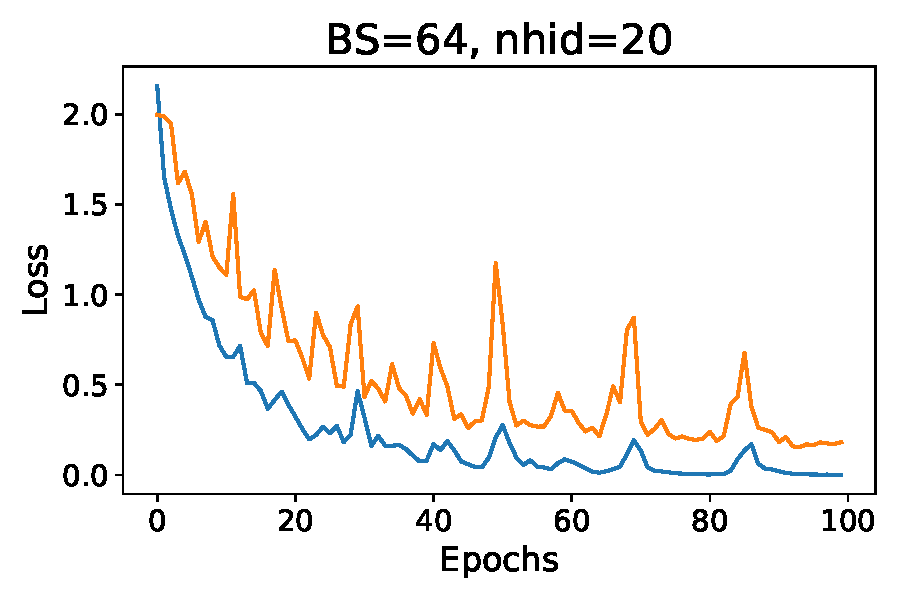
\includegraphics[width=0.7\linewidth]{./Transformer_loss_plot.pdf}
\end{figure}
\par Training logs of the last few steps from three models are reported below, the validation loss of transformer is significantly lower than the previous two decoders. However, the translation results from additive attention is overall better. Additive attention model failed to translate one word (conditioning), but the transformer only translated conditioning correctly, it could be that additive attention works better for short words (because it's recurrent and might suffers from gradient vanishing/exploding problems) but transformer works better for long vocabularies (because it reads the entire sequence the same time).
\begin{lstlisting}
================ GRU ================
Epoch:  95 | Train loss: 0.650 | Val loss: 1.069 | Gen: ethay airway onintoidingsday isway oulgefray
Epoch:  96 | Train loss: 0.647 | Val loss: 1.048 | Gen: ethay ariway onsidtoingray isway oulfrway
Epoch:  97 | Train loss: 0.647 | Val loss: 1.120 | Gen: ethay aringpay ondintingshingbay isway orkingway
Epoch:  98 | Train loss: 0.670 | Val loss: 1.123 | Gen: ethay aringpay onsidtenfay-onsay isway orkgingway
Epoch:  99 | Train loss: 0.673 | Val loss: 1.053 | Gen: ethay aisray onsiditiongray issway oulfreday
================ Additive Attention ================
Epoch:  95 | Train loss: 0.006 | Val loss: 0.138 | Gen: ethay airway onditioningcay isway orkingway
Epoch:  96 | Train loss: 0.006 | Val loss: 0.133 | Gen: ethay airway onditioningcay isway orkingway
Epoch:  97 | Train loss: 0.006 | Val loss: 0.137 | Gen: ethay airway onditioningcay isway orkingway
Epoch:  98 | Train loss: 0.056 | Val loss: 1.192 | Gen: ethay airway ondicecgcay isway orkiwway
Epoch:  99 | Train loss: 0.123 | Val loss: 0.332 | Gen: ethay airway onditionwway isway orkingway
================ Transformer (Enforcing Causal) ================
Epoch:  95 | Train loss: 0.002 | Val loss: 0.166 | Gen: ethhay iarway onditioningcay iseway orkingway
Epoch:  96 | Train loss: 0.002 | Val loss: 0.180 | Gen: ethhay iirway onditioningcay isiiiiiiiiiissssacy orkingwaay
Epoch:  97 | Train loss: 0.002 | Val loss: 0.175 | Gen: ethhay iirway onditioningcay iswway orkingway
Epoch:  98 | Train loss: 0.002 | Val loss: 0.171 | Gen: ethhay iirway onditioningcay iswway orkingway
Epoch:  99 | Train loss: 0.001 | Val loss: 0.182 | Gen: ethhay iirway onditioningcay iswway orkingway
\end{lstlisting}

\subsection{Question 6: Non-causal Decoder}
\par The outputs from the last few training iterations suggested the modified transformer achieves both lower training and validation loss compared with the original transformer. However, the generated translation is non-sense compared with the transformer with causal decoder. The can be resulted from the fact that, without enforcing causal mask, we allow the model to peak into the future, which discourages the decoder from learning the sequential structure of sentences (i.e., the model failed to learn the importance of character orders).
\begin{lstlisting}
================ Output From Transformer with Causal Decoder ================
Epoch:  95 | Train loss: 0.002 | Val loss: 0.166 | Gen: ethhay iarway onditioningcay iseway orkingway
Epoch:  96 | Train loss: 0.002 | Val loss: 0.180 | Gen: ethhay iirway onditioningcay isiiiiiiiiiissssacy orkingwaay
Epoch:  97 | Train loss: 0.002 | Val loss: 0.175 | Gen: ethhay iirway onditioningcay iswway orkingway
Epoch:  98 | Train loss: 0.002 | Val loss: 0.171 | Gen: ethhay iirway onditioningcay iswway orkingway
Epoch:  99 | Train loss: 0.001 | Val loss: 0.182 | Gen: ethhay iirway onditioningcay iswway orkingway
================ Output From Transformer with Normal Decoder ================
Epoch:  95 | Train loss: 0.000 | Val loss: 0.001 | Gen: - - - - -           
Epoch:  96 | Train loss: 0.000 | Val loss: 0.001 | Gen: - - - - -           
Epoch:  97 | Train loss: 0.000 | Val loss: 0.001 | Gen: - - - - -           
Epoch:  98 | Train loss: 0.000 | Val loss: 0.001 | Gen: - - - - -           
Epoch:  99 | Train loss: 0.000 | Val loss: 0.001 | Gen: - - - - -  
\end{lstlisting}
\subsection{Question 7: Advantages and Disadvantages of Additive Attentions and Scaled Dot Product Attention}
\par It seems that the scaled dot attention is better at translating long vocabularies, since a transformer takes the entire sequence of characters once, and can better exploit the correlation between characters distant apart from each other. Additive attention models is based on recurrent neural networks, and RNNs may suffer from vanishing and exploding gradient problems, depends on the specific types of RNN cell used. Therefore, RNN together with additive attentions works better for short vocabularies.


\section{BERT}
\subsection{Question 1}
\par The \texttt{BertCSC413\_MLP} class uses 512 hidden neurones (in contrast to the 768 hidden neurones in the original implementation), and a sigmoid activation function (in contrast to the ReLU activation).
\subsection{Question 2}
\par
\subsection{Question 3}
\begin{figure}[H]
	\centering
	\includegraphics[width=0.5\linewidth]{Inference.png}
\end{figure}
\par These inference tasks involves both standard usages of binary operator (i.e., number + operator + number) and longer compound usages (i.e., using multiple binary operators consecutively). Moreover, three types of representations of numbers are used: plain English(e.g., three), plain numerical (e.g., 3), and English multipliers (e.g., thousand). Interestingly, the model processes ambiguous compound operations differently, for example \texttt{"three minus two minus eight"} is interpreted as $3-2-8 < 0$, but \texttt{"one minus one minus one"} as $1 - (1 - 1) > 0$.
\subsection{Question 4}
\par I changed some hyper-parameters to the training of \texttt{model\_finetune\_bert} by reducing the learning rate while increasing the number of training epochs. Specifically, learning rate is changed to \texttt{5e-5} (originally \texttt{2e-5}) and the model is now trained for 10 epochs (originally 4 epochs). The (overall) validation accuracy improved from 97\% to 98\%, and now the model correctly classifies all samples with negative signs (originally 95.7\%).

\paragraph{Implementation} The code executed, note that I added two keyword arguments to the \texttt{train\_model} method.
\begin{lstlisting}[language=Python]
model_finetune_bert_new = BertCSC413_MLP.from_pretrained(
    "bert-base-uncased", 
    num_labels = 3,    
    output_attentions = False, 
    output_hidden_states = False
)
finttune_bert_loss_vals_new = train_model(model_finetune_bert_new, lr=3e-5, epochs=10)
eval_testdata(model_finetune_bert_new, show_all_predictions=False)
\end{lstlisting}

\paragraph{Validation Logs} The detailed validation logs:
\begin{lstlisting}
==========================================================
				  Old Hyperparameters
==========================================================
Predicting labels for 160 test sentences...
Number of expressions with negative result 47 
 45  predicted correctly , accuracy  0.9574468085106383 

Number of expressions with 0 result 2 
 0  predicted correctly , accuracy  0.0 

Number of expressions with positive result 111 
 111  predicted correctly , accuracy  1.0 

==========================================================
				  New Hyperparameters
==========================================================

Predicting labels for 160 test sentences...
Number of expressions with negative result 47 
 47  predicted correctly , accuracy  1.0 

Number of expressions with 0 result 2 
 0  predicted correctly , accuracy  0.0 

Number of expressions with positive result 111 
 111  predicted correctly , accuracy  1.0 
\end{lstlisting}

\paragraph{Training Logs} The detailed training logs are attached below:
\begin{lstlisting}
==========================================================
				  Old Hyperparameters
==========================================================
======== Epoch 1 / 4 ========
Training...

  Average training loss: 1.08
  Training epcoh took: 0:01:20
Running Validation...
  Accuracy: 0.88
  Validation took: 0:00:01

======== Epoch 2 / 4 ========
Training...

  Average training loss: 0.79
  Training epcoh took: 0:01:19
Running Validation...
  Accuracy: 0.98
  Validation took: 0:00:01

======== Epoch 3 / 4 ========
Training...

  Average training loss: 0.59
  Training epcoh took: 0:01:19
Running Validation...
  Accuracy: 0.97
  Validation took: 0:00:01

======== Epoch 4 / 4 ========
Training...

  Average training loss: 0.53
  Training epcoh took: 0:01:19
Running Validation...
  Accuracy: 0.97
  Validation took: 0:00:01

Training complete!
==========================================================
				  New Hyperparameters
==========================================================
======== Epoch 1 / 10 ========
Training...

  Average training loss: 0.74
  Training epcoh took: 0:01:27
Running Validation...
  Accuracy: 0.73
  Validation took: 0:00:02

======== Epoch 2 / 10 ========
Training...

  Average training loss: 0.47
  Training epcoh took: 0:01:27
Running Validation...
  Accuracy: 0.95
  Validation took: 0:00:02

======== Epoch 3 / 10 ========
Training...

  Average training loss: 0.29
  Training epcoh took: 0:01:28
Running Validation...
  Accuracy: 0.98
  Validation took: 0:00:01

======== Epoch 4 / 10 ========
Training...

  Average training loss: 0.21
  Training epcoh took: 0:01:28
Running Validation...
  Accuracy: 0.98
  Validation took: 0:00:02

======== Epoch 5 / 10 ========
Training...

  Average training loss: 0.18
  Training epcoh took: 0:01:27
Running Validation...
  Accuracy: 0.98
  Validation took: 0:00:01

======== Epoch 6 / 10 ========
Training...

  Average training loss: 0.15
  Training epcoh took: 0:01:28
Running Validation...
  Accuracy: 0.98
  Validation took: 0:00:02

======== Epoch 7 / 10 ========
Training...

  Average training loss: 0.13
  Training epcoh took: 0:01:28
Running Validation...
  Accuracy: 0.98
  Validation took: 0:00:02

======== Epoch 8 / 10 ========
Training...

  Average training loss: 0.13
  Training epcoh took: 0:01:28
Running Validation...
  Accuracy: 0.98
  Validation took: 0:00:02

======== Epoch 9 / 10 ========
Training...

  Average training loss: 0.12
  Training epcoh took: 0:01:28
Running Validation...
  Accuracy: 0.98
  Validation took: 0:00:01

======== Epoch 10 / 10 ========
Training...

  Average training loss: 0.12
  Training epcoh took: 0:01:28
Running Validation...
  Accuracy: 0.98
  Validation took: 0:00:02

Training complete!
\end{lstlisting}
\end{document}





















